\documentclass[a4paper,12pt]{article}
%\documentclass{Configuration_Files/Template}

%------------------------------------------------------------------------------
%	REQUIRED PACKAGES AND  CONFIGURATIONS
%------------------------------------------------------------------------------

% CONFIGURATIONS
\usepackage{parskip} % For paragraph layout
\usepackage{setspace} % For using single or double spacing
\usepackage{emptypage} % To insert empty pages
\usepackage{multicol} % To write in multiple columns (executive summary)
\setlength\columnsep{15pt} % Column separation in executive summary
\setlength\parindent{0pt} % Indentation
\raggedbottom  

% PACKAGES FOR TITLES
\usepackage{titlesec}
% \titlespacing{\section}{left spacing}{before spacing}{after spacing}
\titlespacing{\section}{0pt}{3.3ex}{2ex}
\titlespacing{\subsection}{0pt}{3.3ex}{1.65ex}
\titlespacing{\subsubsection}{0pt}{3.3ex}{1ex}
\usepackage{color}

% PACKAGES FOR LANGUAGE AND FONT
\usepackage[english]{babel} % The document is in English  
\usepackage[utf8]{inputenc} % UTF8 encoding
\usepackage[T1]{fontenc} % Font encoding
\usepackage[11pt]{moresize} % Big fonts

% PACKAGES FOR IMAGES
\usepackage{graphicx}
\usepackage{transparent} % Enables transparent images
\usepackage{eso-pic} % For the background picture on the title 
\usepackage{rotating}
\usepackage{subfig} % Numbered and caption subfigures using \subfloat.
\usepackage{tikz} % A package for high-quality hand-made figures.
\usetikzlibrary{}
\graphicspath{{./Images/}} % Directory of the images
\usepackage{caption} % Coloured captions
\usepackage{amsthm,thmtools,xcolor} % Coloured "Theorem"
\usepackage{float}

% STANDARD MATH PACKAGES
\usepackage{amsmath}
\usepackage{amsthm}
\usepackage{amssymb}
\usepackage{amsfonts}
\usepackage{bm}
\usepackage[overload]{empheq} % For braced-style systems of equations.
\usepackage{fix-cm} % To override original LaTeX restrictions on sizes

% PACKAGES FOR TABLES
\usepackage{tabularx}
\usepackage{longtable} % Tables that can span several pages
\usepackage{colortbl}

% PACKAGES FOR ALGORITHMS (PSEUDO-CODE)
\usepackage{algorithm}
\usepackage{algorithmic}

% PACKAGES FOR REFERENCES & BIBLIOGRAPHY
\usepackage[colorlinks=true,linkcolor=black,anchorcolor=black,citecolor=black,filecolor=black,menucolor=black,runcolor=black,urlcolor=black]{hyperref} % Adds clickable links at references
\usepackage{cleveref}
\usepackage[square, numbers, sort&compress]{natbib} % Square brackets, citing references with numbers, citations sorted by appearance in the text and compressed
\bibliographystyle{abbrvnat} % You may use a different style adapted to your field

% OTHER PACKAGES
\usepackage{pdfpages} % To include a pdf file
\usepackage{afterpage}
\usepackage{lipsum} % DUMMY PACKAGE
\usepackage{fancyhdr} % For the headers
\fancyhf{}

%----------------------------------------------------------------------------
%	NEW COMMANDS DEFINED
%----------------------------------------------------------------------------

% EXAMPLES OF NEW COMMANDS
\newcommand{\bea}{\begin{eqnarray}} % Shortcut for equation arrays
\newcommand{\eea}{\end{eqnarray}}
\newcommand{\e}[1]{\times 10^{#1}}  % Powers of 10 notation

%----------------------------------------------------------------------------
%	ADD YOUR PACKAGES (be careful of package interaction)
%----------------------------------------------------------------------------

\usepackage{geometry}
\usepackage{tabularx}
\usepackage{booktabs,xltabular}

%----------------------------------------------------------------------------
%	ADD YOUR DEFINITIONS AND COMMANDS (be careful of existing commands)
%----------------------------------------------------------------------------

% Set uniform margins
\geometry{
  left=0.8in,
  right=0.8in,
  top=1in,
  bottom=1in,
  includehead,
  includefoot
}

\begin{document}
\title{Students\&Company Design Document} % Title Page
\author{Alessandro Salvatore, Erdal Yalçın, Leonardo Ratti}
\date{Academic Year: 2024-25}
\maketitle

\tableofcontents
\newpage

\section{Introduction}
\subsection{Purpose}
\subsubsection{Goals}
\subsection{Scope}
\subsubsection{Definitions}
\subsubsection{Acronyms}
\subsubsection{Abbreviations}
\subsection{Revision History}
\subsection{Reference Documents}
\subsection{Document Structure}

\section{Overall Description}
\subsection{Overview: High-level Components and Interaction}
\subsection{Component View}
In this section we show the components and their relationships. The following
sections will explain the interaction between interfaces and details on each method of interfaces.
\begin{figure}[H]
\centering
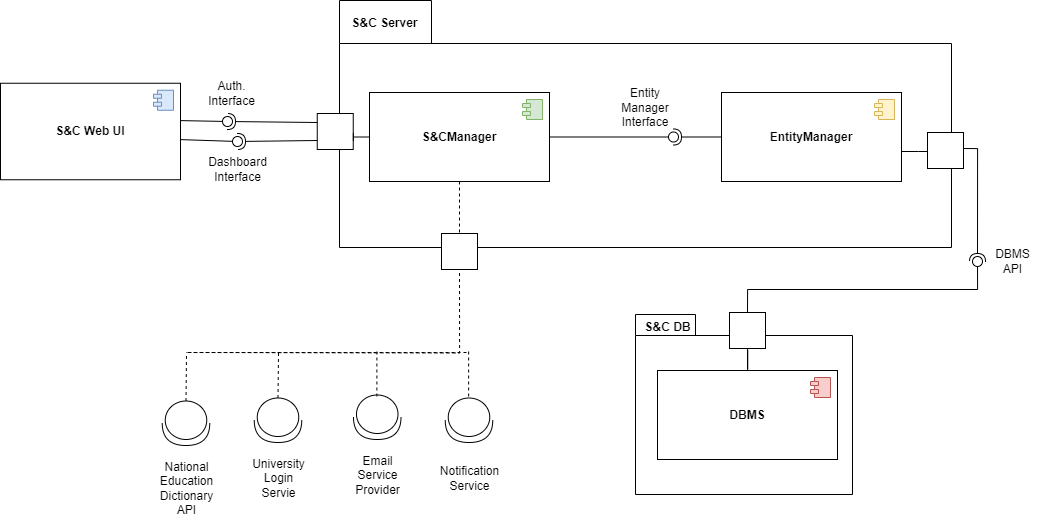
\includegraphics[scale = 0.50]{DD_images/GeneralComponentDiagram.drawio.png}\\
\caption{Component Diagram of the Student\&Companies System}
\end{figure}

\subsubsection{Entity Manager}
This component is responsible for communication with a Database Management System (DBMS).
It follows the Adapter design pattern, allowing other components to interact with the DBMS
without needing to write any SQL code themselves.
\subsubsection{S\&C-SP}
The S\&CSP subsystem implements S\&C's logic. It provides all the system's features, including the recommendation system.
\begin{sidewaysfigure}% Use sidewaysfigure instead of figure
\centering
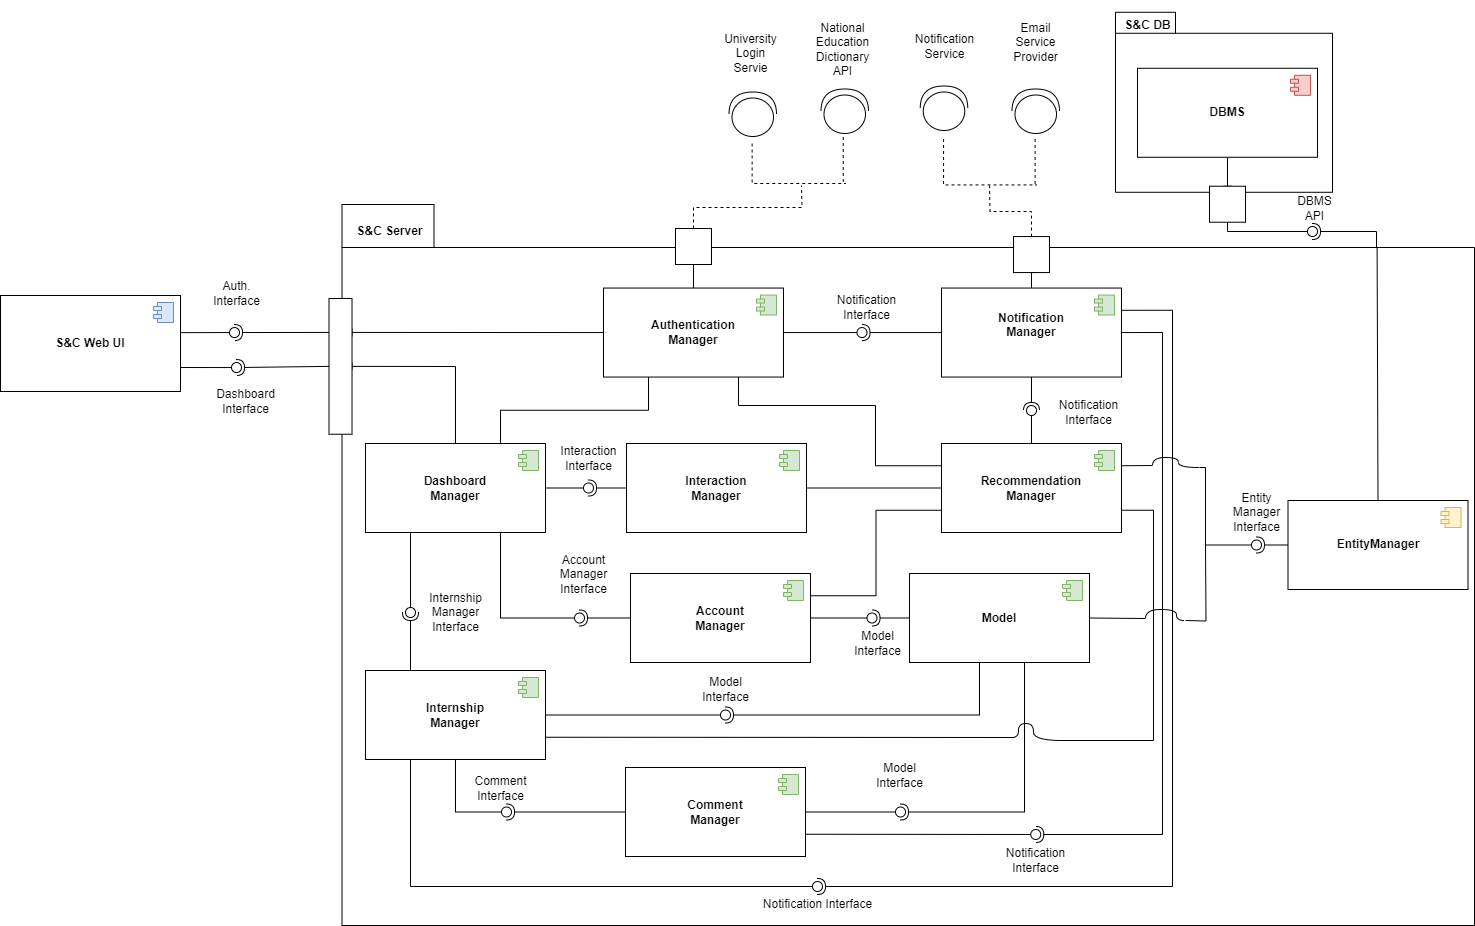
\includegraphics[scale=0.50]{DD_images/S&C.drawio.png}\\
\caption{Component Diagram of the S\&C-SP subsystem}
\end{sidewaysfigure}
\begin{enumerate}
    \item {Dashboard Manager} :
    \\It's used as an intermediary between the WebUI and the
    other components of the server to provide the web application only the functionality
    strictly necessary for it to work properly.
    \item {Account Manager} :
    \\This component handles the operations needed to manage each User's account, and to view the Users' profiles. It allows Users to login, using the Authentication Manager's interface.
    \item {Authentication Manager} :
    \\This component handles signup, login and logout operations.
    \item {Internship Manager} :
    \\This component handles the operations needed to manage an Internship, to view any information about it and to accept it.
    \item {Comment Manager} :
    \\This component handles the operations needed to view and write comments (complaints and observations.
    \item {Recommendation Manager} :
    \\This component is responsible for the recommendation mechanism for students and internships. It takes the input data from the user interactions with the system and reloads the associated recommendations.
    \item {Interaction Manager} :
    \\This component is responsible for registering feedbacks and interactions of the user with the web application, transforming this information into parameters, and passing it to the recommendation manager for elaboration.
    \item {Notification Manager} :
    \\This component is responsible for the dispatch of notifications.
    \item {Model} :
    \\This component facilitates the interaction with and representation of S\&C-SP data.
\end{enumerate}
\subsection{Deployment View}
We adopted a 3-tier architecture hosted on cloud infrastructure, designed to optimize performance and scalability while reducing costs.

Let's explore more in detail:

\begin{enumerate}
    \item \textbf{Scalability and Flexibility} - the ability to add or remove resources such as virtual machines, performance cores, or memory as needed, in conjunction with the use of load balancing services, allows the servers to adapt to changes in traffic or workload.
    \item \textbf{Security} - Firewalls help to protect the application server against data breaches and other security threats.
    \item \textbf{Cost-efficiency} - the choice of using a cloud provider allows us to only pay for the resources that we are actually using, which can help to lower the overall costs, and in general reduces the waste of resources.
\end{enumerate}

The cloud provider is an ideal choice for hosting large, high-traffic applications. The chosen cloud provider will need to offer all of these features in order to meet our needs.

The web server resides in the De Militarized Zone and is the primary interface for user interaction. The application server executes the core application logic, processing user requests and handling all the operations. Load balancers are implemented to evenly distribute incoming traffic across multiple instances of Web and Application Servers.
\begin{figure}[H]
    \centering
    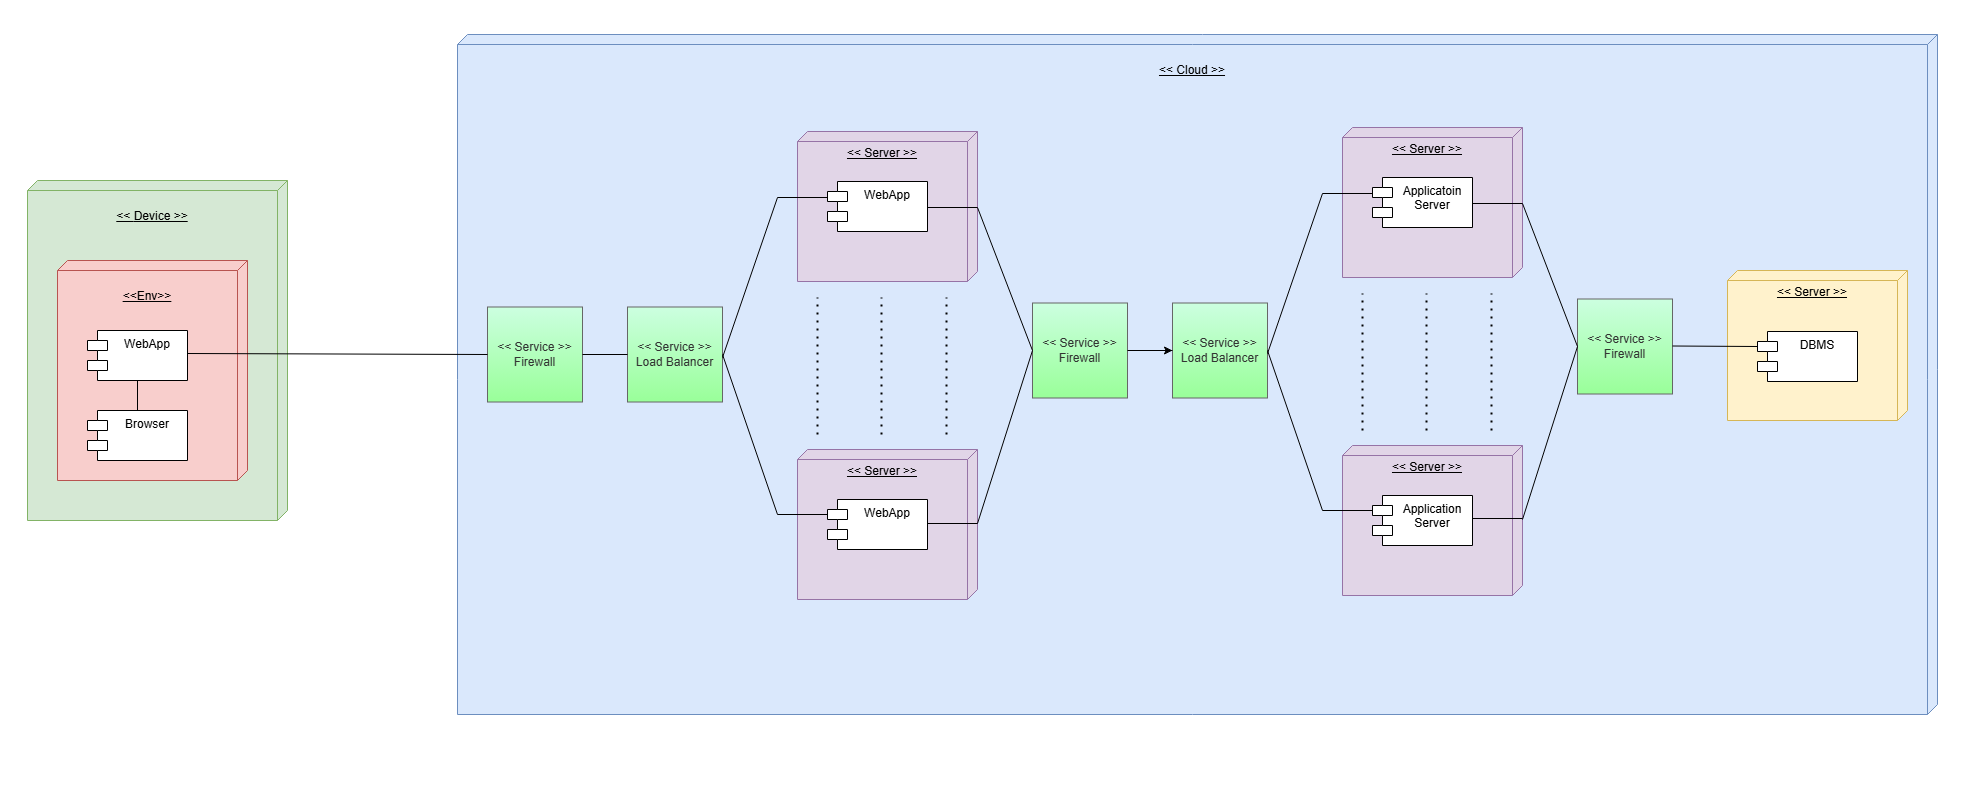
\includegraphics[scale = 0.33]{figures/DD/SingleDiagrams/DeploymentView.png}
    \caption{University Sign Up Page}
    \centering
\end{figure}
\subsection{Runtime View}
\subsection{Component Interfaces}
\subsubsection{API Endpoints}
\subsection{Selected Architectural Styles and Patterns}
\subsection{Other Design Decisions}
\subsubsection{Scale-out}
\subsubsection{Relational Database}
\subsubsection{Token-Based Authentication and Authorization}
\subsubsection{Distributed MVC Pattern}

\section{User Interface Design}

\section{Requirements Traceability}

\section{Implementation, Integration and Testing Plan}
\subsection{Development Process and Approach}
\subsection{Implementation \& Integration Plan}
\subsubsection{Server Side}
\subsubsection{Client Side}
\subsubsection{Final Integration Test}
\subsection{Technologies}
\subsubsection{Development Technologies}
\subsubsection{Testing Technologies}

\section{Effort Spent}
\subsection{Effort Spent per Unit}

\section{References}
\subsection{References and Tools}

\end{document}
